\begin{figure}[htbp]
\centering 
  \subfloat[Box plot \acs{SCT}.]{
	  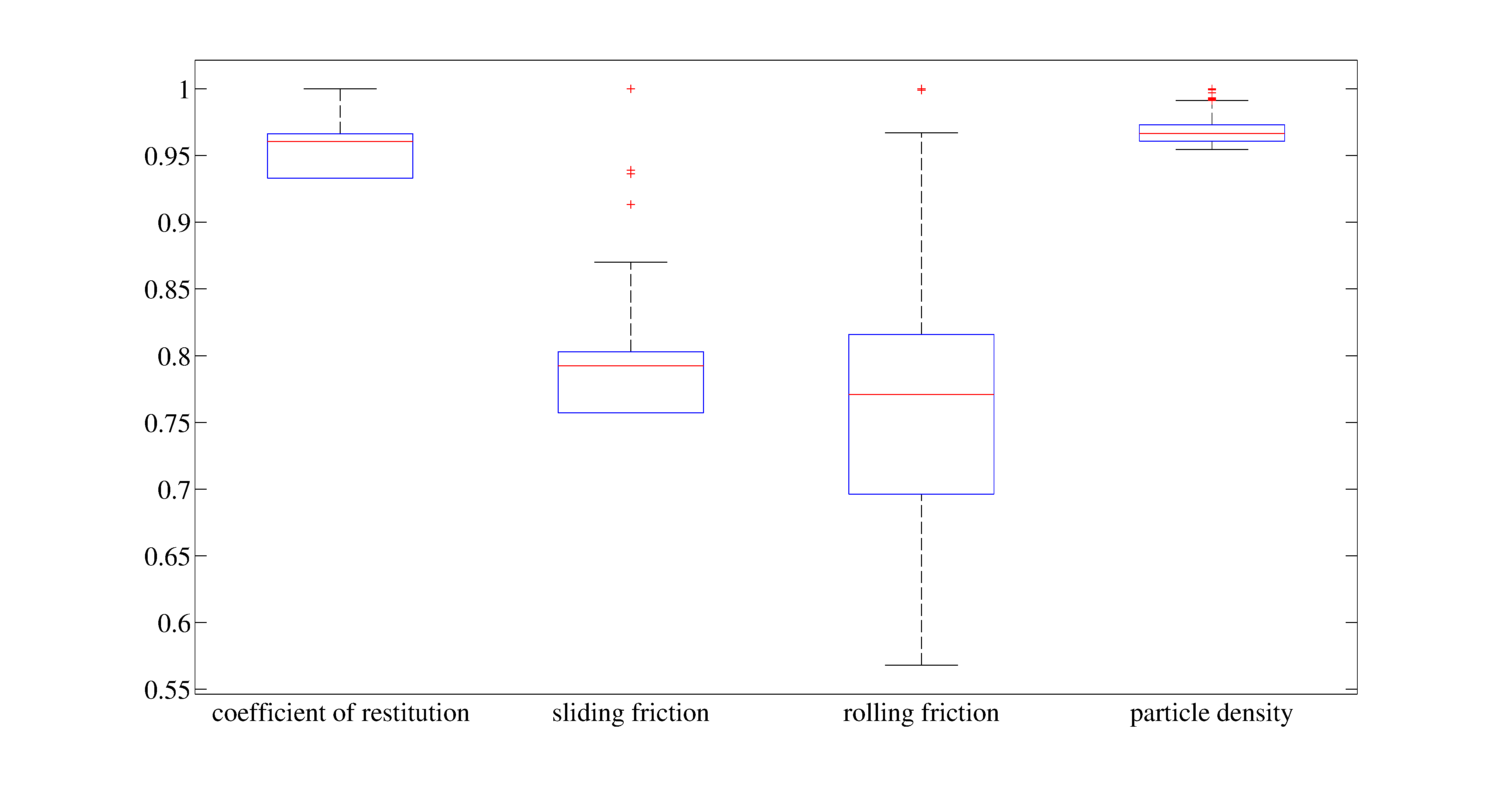
\includegraphics[width=.47\columnwidth]{images/164BoxSCTlimestonecoarsetest01coeffP1}
	  \label{fig:164BoxSCTlimestonecoarsetest01coeffP1}
  }
  \quad
  \subfloat[Density plot \acs{SCT}.]{
	  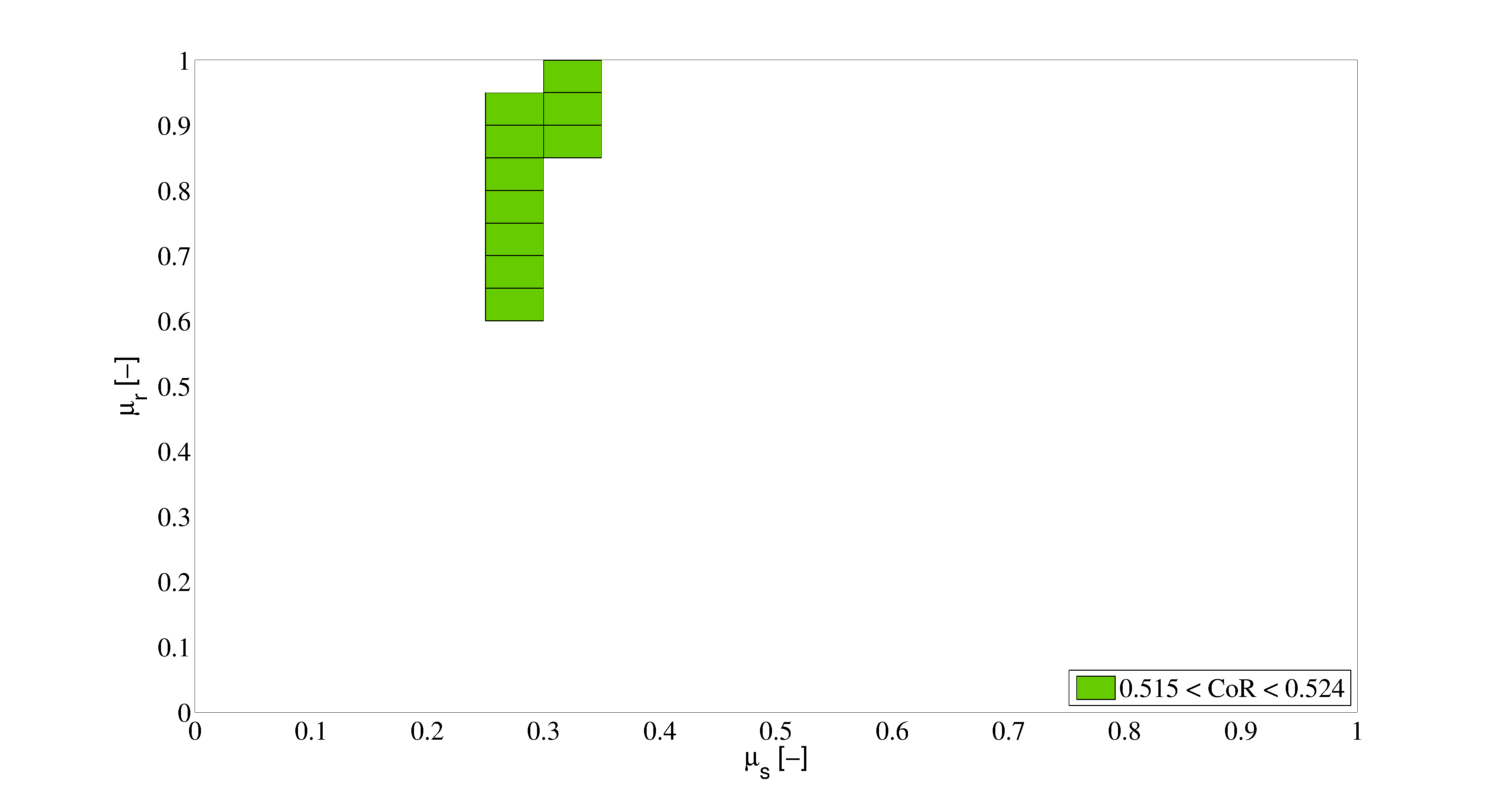
\includegraphics[width=.47\columnwidth]{images/170TileSClimestonecoarsetest01co36-10}
	  \label{fig:170TileSClimestonecoarsetest01co36-10}
  }
  \\
    \subfloat[Box plot \acs{AoR}.]{
	  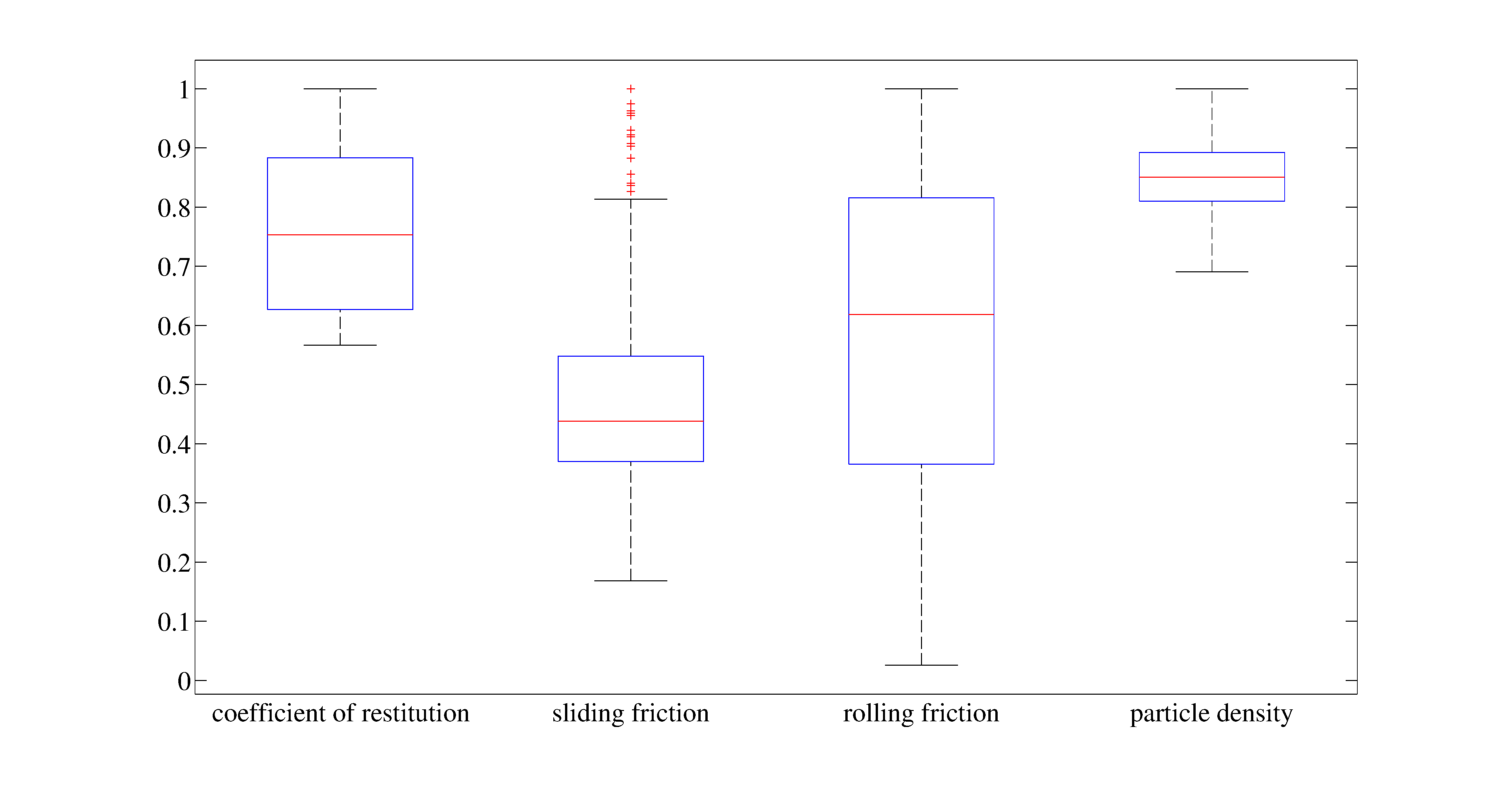
\includegraphics[width=.47\columnwidth]{images/185BoxAORlimestonecoarse}
	  \label{fig:185BoxAORlimestonecoarse}  }
  \quad
  \subfloat[Density plot \acs{AoR}.]{
	  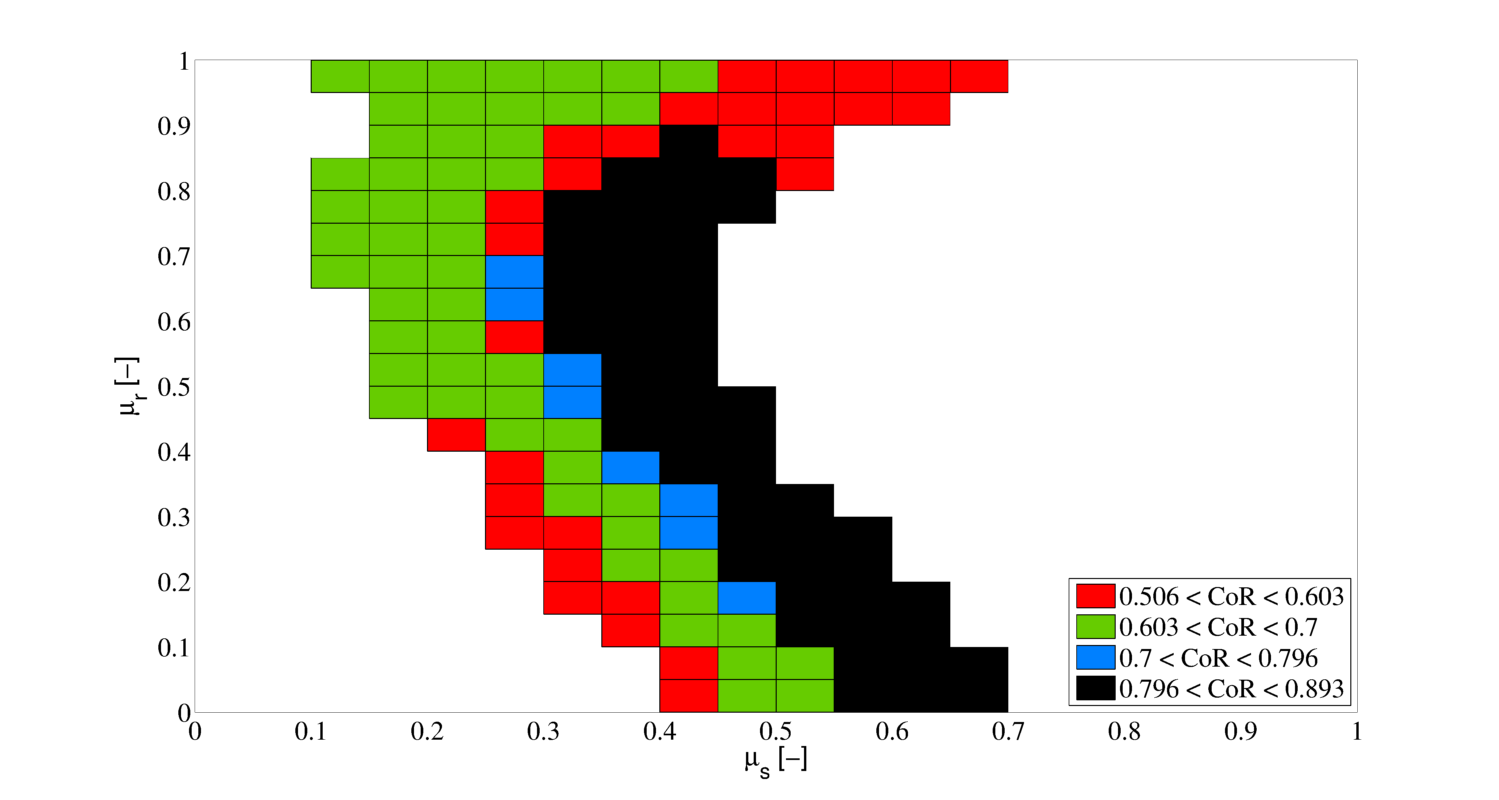
\includegraphics[width=.47\columnwidth]{images/186TileAORlimestonecoarse}
	  \label{fig:186TileAORlimestonecoarse}  }
  \\
  \subfloat[Box plot intersection: \acs{AoR} \& \acs{SCT}.]{
	  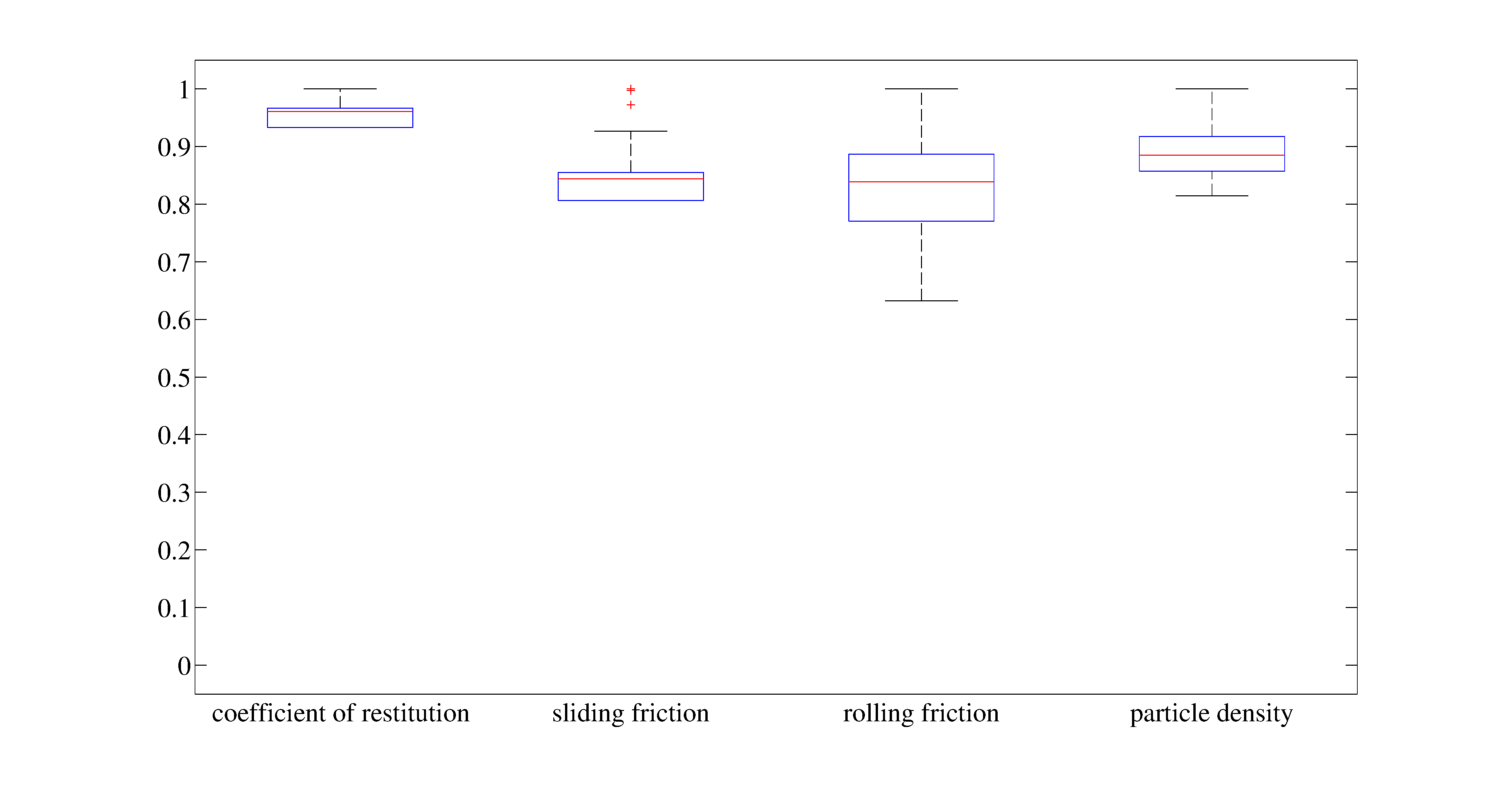
\includegraphics[width=.47\columnwidth]{images/193BoxMixlimestonecoarse_14}
	  \label{fig:193BoxMixlimestonecoarse_14}
  }
  \quad
  \subfloat[Density plot intersection: \acs{AoR} \& \acs{SCT}.]{
	  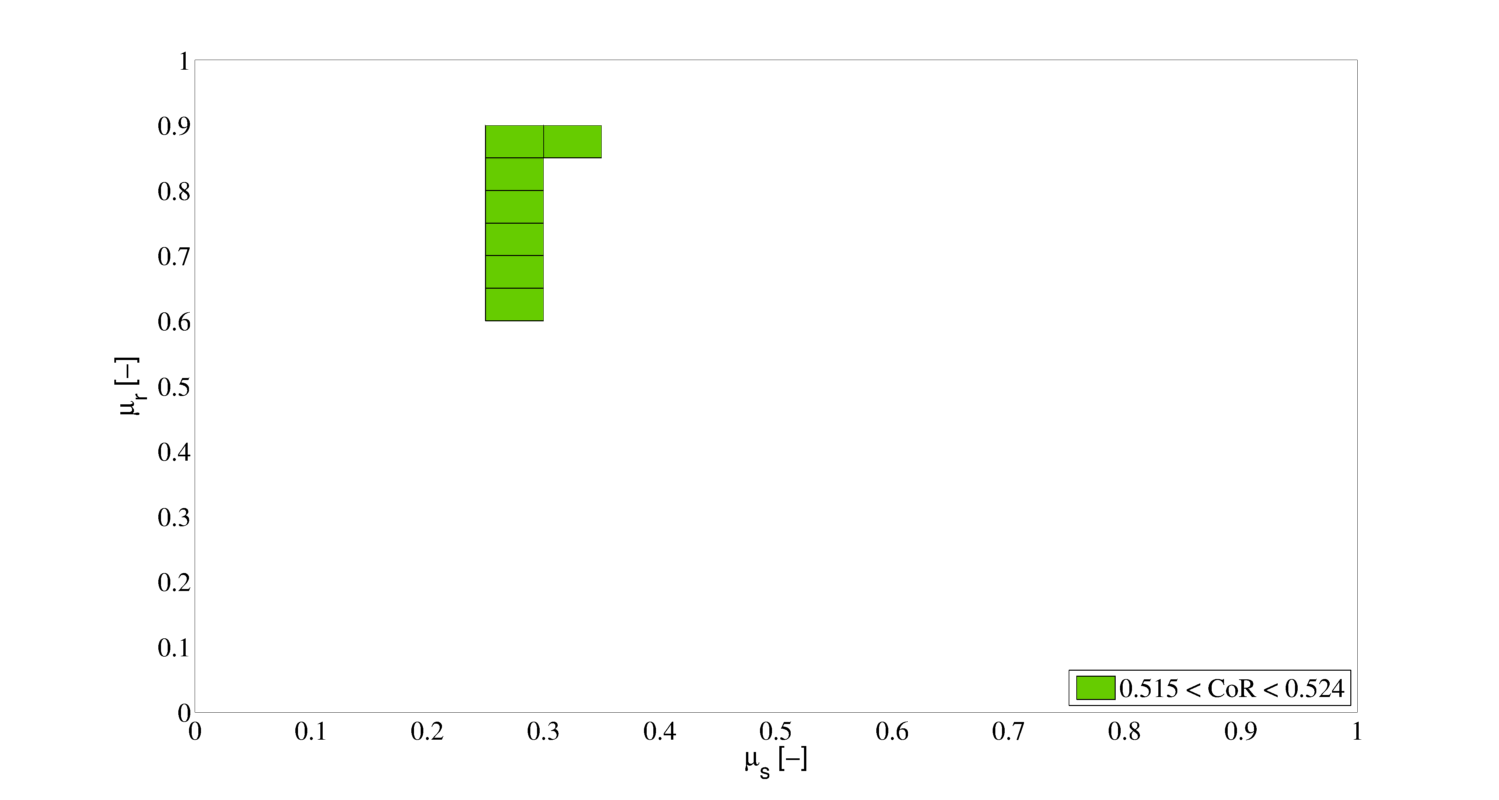
\includegraphics[width=.47\columnwidth]{images/194TileMixlimestonecoarse_14}
	  \label{fig:194TileMixlimestonecoarse_14}
  }
  \\  
  \caption[Limestone coarse valid values]{Limestone coarse valid values. The
  valid values for the \acs{SCT} and \acs{AoR} tests are shown, together with the merge values, valid for both.
  The plots referring to the single test show reasonably narrow confidence
  ranges, while Fig. \ref{fig:193BoxMixlimestonecoarse_14} shows unreasonably large
  valid ranges. See Section \ref{sec:remainingmaterialscharacterization} for
  the interpretation.}
  \label{fig:217boxplotslimestonecoarse}
\end{figure}